\chapter{Operating Systems Services}

\section{Operating System Services}

    Operating systems provide an environment for execution of programs and services to programs and users. The principal services that an operating system provides are:
    \begin{itemize}
        \item \textbf{User Interfaces:} Almost all operating systems have a user interface (UI). The UI can be a command-line interface (CLI), in which the user types commands, or a graphical user interface (GUI), in which the user interacts with the system through graphical elements such as windows, icons, and menus, touch screens, etc.
        \item \textbf{Program Execution:} The system must be able to load a program into memory and to run that program. The program must be able to end its execution, either normally or abnormally (indicating error).
        \item \textbf{I/O Operations:} A program may require I/O, which involve a file or a device.
        \item \textbf{File System Manipulation:} The file system provides the abstraction of a file, which is a collection of related information defined by its creator. The operating system must provide the mechanisms for creating, deleting, reading, writing, and manipulating files and directories.
        \item \textbf{Communications:} Processes may exchange information, on the same computer or between computers over a network. The communication may be implemented through \emph{shared memory} or through \emph{message passing}.
        \item \textbf{Error Detection:} The OS needs to be constantly aware of possible errors: in the CPU and memory hardware, in I/O devices, in the user program. The OS should take the appropriate action to ensure correct and consistent computing. \emph{Debugging} facilities can greatly enhance the user's and programmer's abilities to efficiently use the system.
    \end{itemize}
    Another set of OS functions exists for ensuring the efficient operation of the system itself via \emph{resource sharing}:
    \begin{itemize}
        \item \textbf{Resource Allocation:} When multiple users or multiple jobs run concurrently, resources must be allocated to each of them. If the resources are not sufficient to satisfy the needs of all users, the OS must have a method of deciding between conflicting requests.
        \item \textbf{Logging:} To keep track of which users use the system, what resources they use, and how much time they use them, the OS must maintain a log of such information.
        \item \textbf{Protection:} When multiple processes share the same computer, it is essential to ensure that one process does not interfere with another process or with the OS itself. Protection involves both hardware and software mechanisms that control access to system resources.
        \item \textbf{Security:} Security of the system from outsiders is provided by means of passwords and similar techniques. The OS must ensure that external I/O devices (e.g., a modem) are protected from external interference.
    \end{itemize}


\begin{figure}[H]
    \centering
    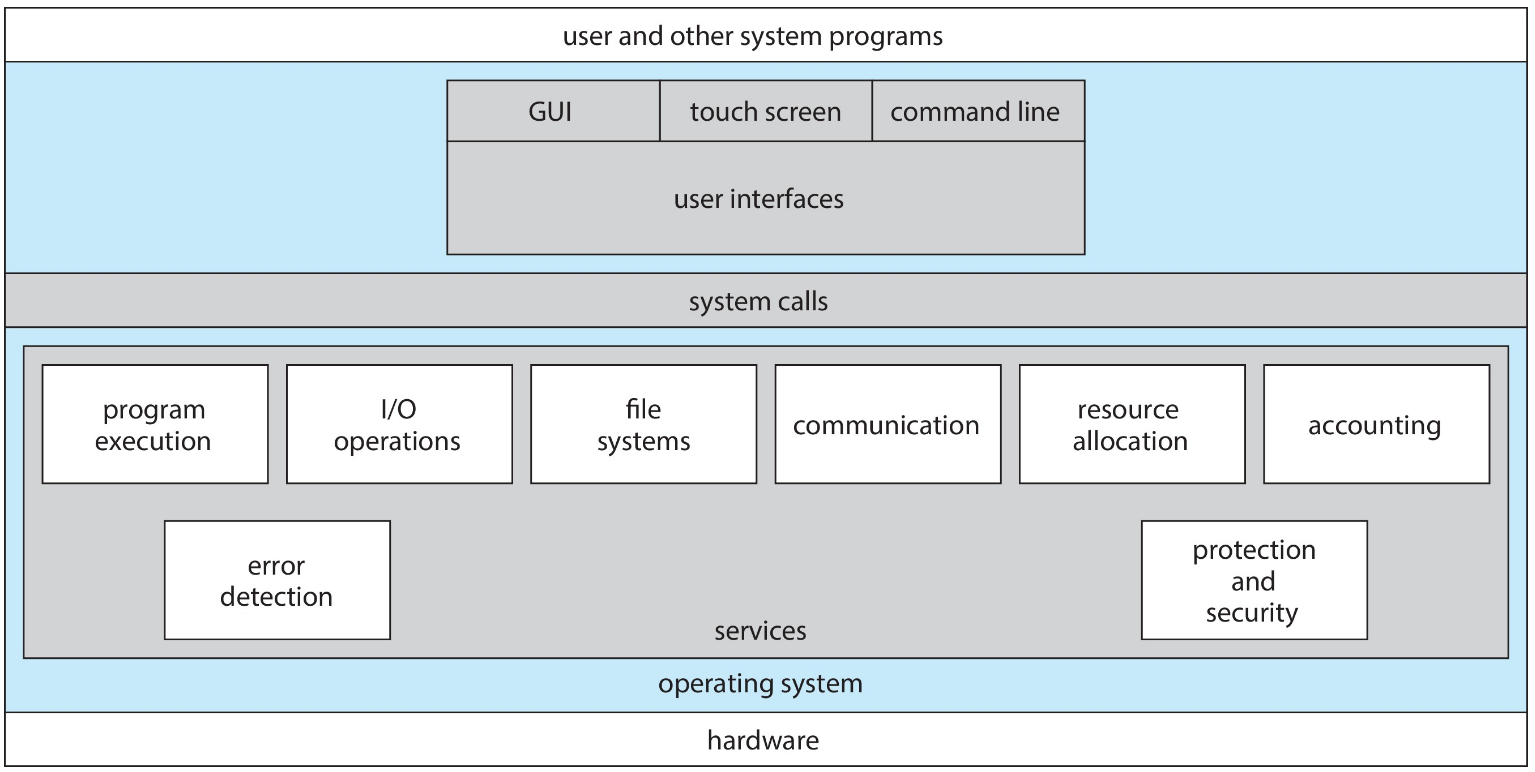
\includegraphics[width=0.8\textwidth]{images/OS_services.png}
    \caption{A View of Operating System Services}
    \label{fig:os_services}
\end{figure}

\section{System Services}

    System programs provide a convenient environment for program development and execution. They can be divided into:
    \begin{itemize}
        \item \textbf{File Manipulation:} Create, delete, copy, rename, print, dump, list, and generally manipulate files and directories.
        \item \textbf{Status Information:} Some programs ask the system for information such as date, time, available memory, disk space, and number of users. Others provide detailed performance, logging, and debugging information. Typically, these programs format and print the output to the terminal or other output devices. Some systems implement a \emph{registry}, used to store and retrieve configuration information.
        \item \textbf{File Modification:} Text editors to create and modify files; special commands to search contents of files or perform transformations of the text.
        \item \textbf{Programming Language Support:} Compilers, assemblers, debuggers, and interpreters may be provided by the system.
        \item \textbf{Program Loading and Execution:} Absolute loaders, relocatable loaders, linkage editors, overlay-loaders, and debugging systems for higher-level and machine language programs.
        \item \textbf{Communications:} Provide the mechanisms for creating virtual connections among processes, users, and computer systems. Allow users to send messages, browse web pages, send e-mails, log in remotely, or transfer files between machines.
        \item \textbf{Background Services:} Launch at boot time. Some run during system startup and then terminate, while others remain active until shutdown. They provide facilities like disk checking, process scheduling, error logging, and printing. These programs run in user context (not kernel context) and are known as services, subsystems, or \emph{daemons}.
        \item \textbf{Application Programs:} Do not pertain directly to the operating system. They are run by users (e.g., productivity software, games) and launched via command line, mouse click, or touchscreen input.
    \end{itemize}
    Most users’ view of the operating system is defined by these \textbf{system programs}, not by the actual system calls.


\subsection{Linkers and Loaders}

    When source code is compiled, it is first translated into \textbf{object files}, which are typically relocatable. A relocatable object file is designed so that its code and data can be loaded into any physical memory address, without being fixed in advance.

    The task of the \textbf{linker} is to combine these object files into a single \textbf{executable binary file}. During this process, the linker resolves external references (for example, function calls that are defined in another file) and incorporates necessary parts of system libraries. In this way, a complete program image is produced, ready to be loaded into memory.

    The executable file, however, still resides on secondary storage. To be executed, it must be brought into main memory by the \textbf{loader}. The loader assigns the final memory addresses to the different parts of the program and adjusts code and data so that they can be correctly accessed during execution. This step is called \emph{relocation}.

    Modern operating systems often rely on \textbf{dynamic linking} instead of including full copies of libraries inside each executable. With dynamic linking, libraries (Windows: \emph{DLLs}, Linux: \emph{shared objects, SOs}) are loaded into memory only once and shared by all programs that use them. This approach saves memory and makes it easier to update libraries without recompiling applications.

    Finally, both object and executable files follow well-defined \textbf{standard formats} (such as ELF in Linux or PE in Windows). Thanks to these formats, the operating system can understand how to correctly load a program into memory and start its execution.



\begin{figure}[H]
    \centering
    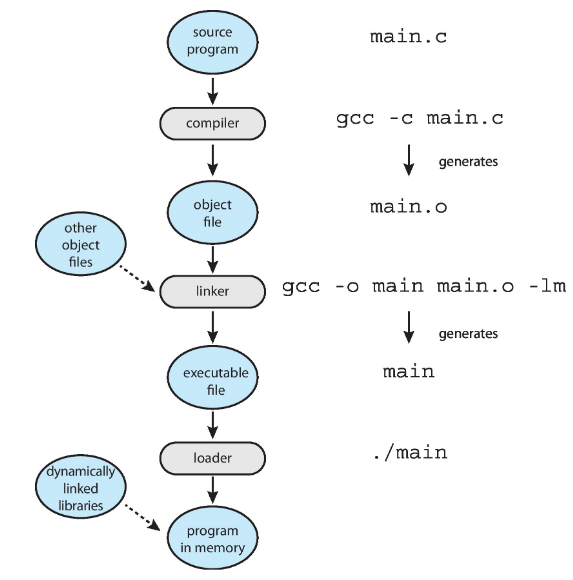
\includegraphics[width=0.5\textwidth]{images/Linker_Loader.png}
    \caption{The Role of the Linker and Loader}
    \label{fig:linker_loader}
\end{figure}


    In the examples below, we compare two very different approaches to system design.  
    
    A system with no operating system is typically single-tasking. Programs, often called sketches, are loaded via USB into flash memory. The entire system uses a single memory space, and a simple boot loader is responsible for loading the program at startup. When a program exits, control does not return to an operating system but instead to the sketch loop, which is executed again. In this environment, the program essentially becomes the system itself, with minimal support beyond the hardware and boot loader. This model is common in microcontrollers and embedded systems.
    
    In contrast, FreeBSD represents a more sophisticated design as a Unix variant that supports multitasking. When the system starts, users log in and invoke their choice of shell. The shell then executes the \texttt{fork()} system call to create a new process and uses \texttt{exec()} to load a program into that process. The shell may wait for the process to terminate or continue handling user commands in parallel. When a process terminates, it returns an exit code: a code of zero indicates that no error occurred, while a value greater than zero indicates an error condition. This model illustrates how modern multitasking operating systems manage processes, provide controlled execution, and report errors in a structured way.
    
    

\begin{figure}[H]
    \centering
    \begin{minipage}{0.3\textwidth}
        \centering
        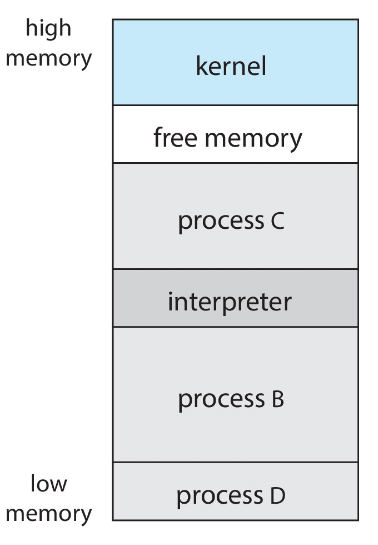
\includegraphics[width=\textwidth]{images/FreeBSD.png}
        \caption{Example: FreeBSD}
        \label{fig:example_freebsd}
    \end{minipage}
    \hfill
    \begin{minipage}{0.4\textwidth}
        \centering
        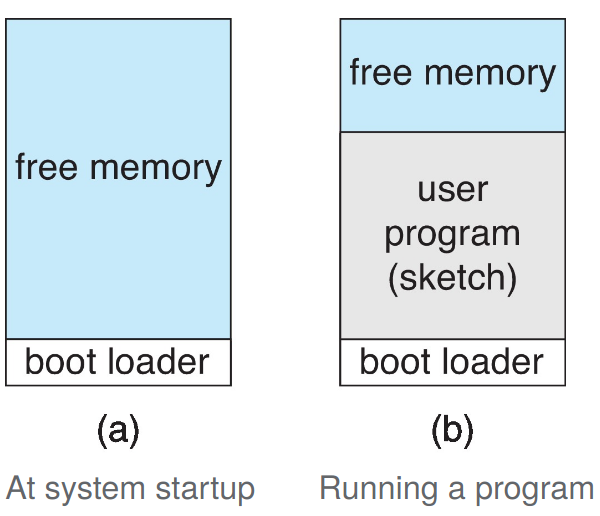
\includegraphics[width=\textwidth]{images/Arduino.png}
        \caption{Example: Arduino}
        \label{fig:example_arduino}
    \end{minipage}
    \label{fig:dual_vs_symmetric}
\end{figure}

\section{System Calls}

    A compiled program cannot be executed by different operating system, the principal reason are:
    \begin{itemize}
        \item Different operating systems have different system calls.
        \item Different \emph{Application Binary Interfaces} (ABIs), wich define how different components of binary code can interface for a given operating system on a given architecture, CPU, etc.
        \item Different executable file formats.
        \item Different ISA and hardware architectures. This example not depending on the operating system, but on the CPU architecture.
    \end{itemize}
    To solve this problem we have two principal methods:
    \begin{itemize}
        \item \textbf{interpreters:} we write code in a high-level language, and then we use an interpreter to execute the code. The interpreter is a program that reads the high-level code and translates it into machine code on-the-fly, allowing the same high-level code to run on different operating systems and architectures. This approach is common for scripting languages like Python, JavaScript, and Ruby. Obliviously, the interpreter itself must be available for each target operating system and architecture.
        \item \textbf{virtual machines:} a virtual machine (VM) is a software emulation of a physical computer that runs an operating system and applications. The VM provides a consistent environment for running programs, regardless of the underlying hardware and operating system. Examples of VMs include the Java Virtual Machine (JVM) and the .NET Common Language Runtime (CLR).
    \end{itemize}


    The programming interface to the services provided by the operating system is typically written in a high-level language such as C or C++. In most cases, these services are accessed by programs through a high-level Application Programming Interface (API) rather than by making direct use of system calls. The three most common APIs are the Win32 API for Windows, the POSIX API for POSIX-based systems (which include virtually all versions of UNIX, Linux, and macOS), and the Java API for the Java Virtual Machine (JVM). It is important to note that the system-call names used throughout this presentation are generic and may differ across specific implementations.


\begin{figure}[H]
    \centering
    \begin{minipage}{0.5\textwidth}
        \centering
        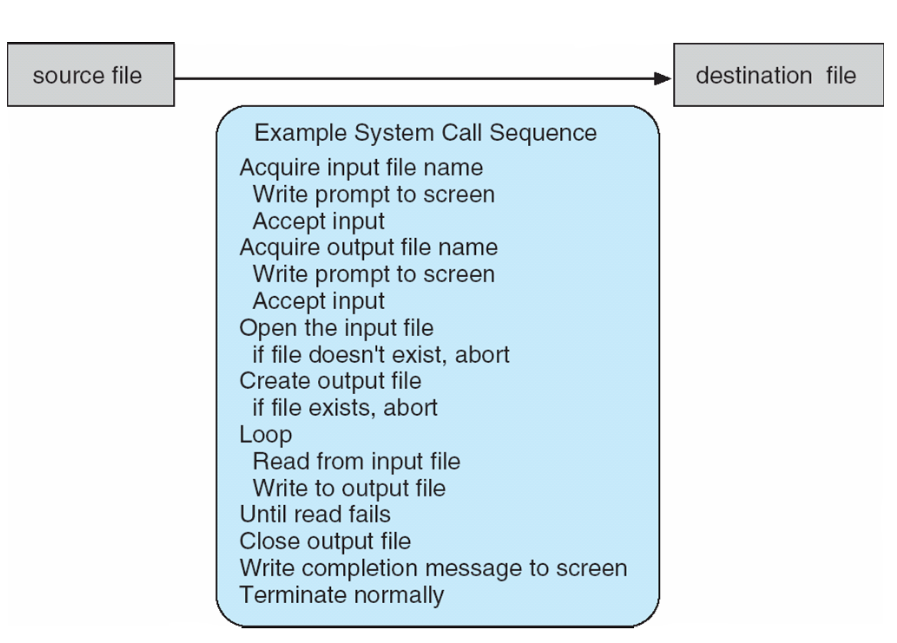
\includegraphics[width=\textwidth]{images/SYC_example.png}
        \caption{Example: System call for copy the contents of a file to another file}
        \label{fig:example_syc}
    \end{minipage}
    \hfill
    \begin{minipage}{0.45\textwidth}
        \centering
        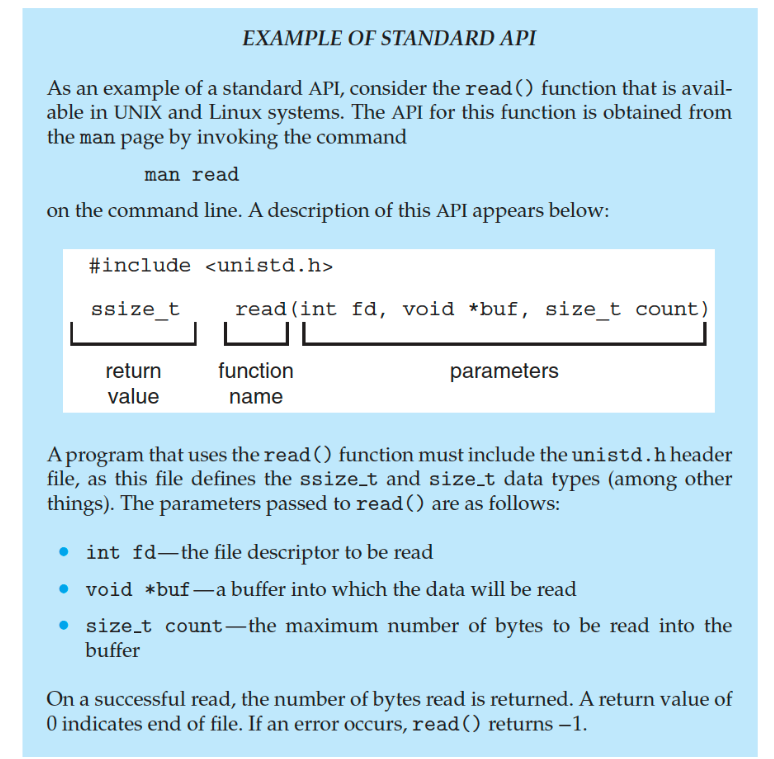
\includegraphics[width=\textwidth]{images/Standard_API.png}
        \caption{Example: Read standard API}
        \label{fig:Example standard api}
    \end{minipage}
    \label{fig:example_api}
\end{figure}

\subsection{System Call Implementation}

Typically, a number is associated with each system call. The system-call interface maintains a table indexed according to these numbers, which it uses to invoke the intended system call in the OS kernel. After execution, the interface returns the status of the system call along with any return values to the caller. The programmer does not need to know how the system call is implemented internally; it is sufficient to follow the API and understand what the operating system will do as a result of the call. Most details of the OS interface are hidden from the programmer by the API, and the entire process is managed by a run-time support library, which is a set of functions built into the libraries included with the compiler.



\begin{figure}[H]
    \centering
    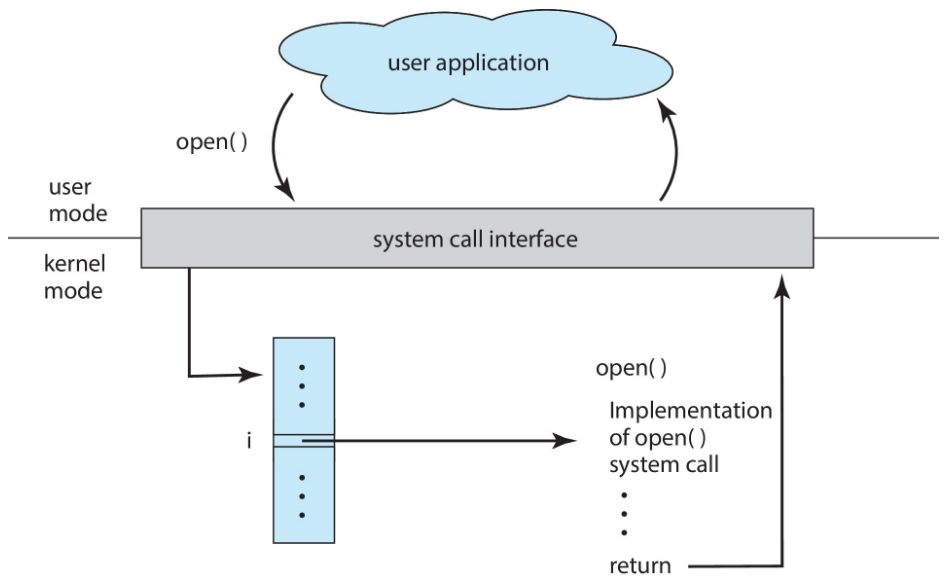
\includegraphics[width=0.6\textwidth]{images/API-SYC.png}
    \caption{System Call Implementation}
    \label{fig:api_syc}
\end{figure}

\subsection{System Call Parameter Passing}

    There are three general methods for passing parameters to the operating system when a system call is made:
    \begin{itemize}
        \item \textbf{Registers:} The parameters are stored in registers and passed to the OS kernel. This method is fast but limited by the number of available registers.
        \item \textbf{Block or Table:} The parameters are stored in a block or table in memory, and the address of this block is passed to the OS kernel in a register. This method allows for more parameters to be passed but requires additional memory access.
        \item \textbf{Stack:} The parameters are pushed onto the stack by the program and popped off the stack by the OS kernel. This method is flexible and can handle a variable number of parameters, but it may be slower due to stack operations.
    \end{itemize}
    The choice of parameter-passing method depends on factors such as the architecture of the CPU, the design of the operating system, and performance considerations.



\begin{figure}[H]
    \centering
    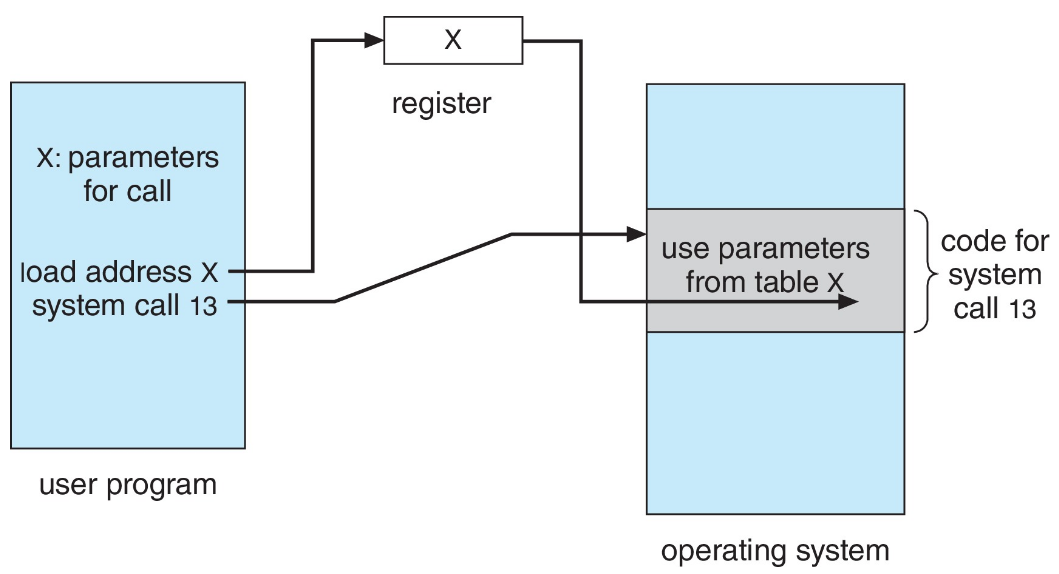
\includegraphics[width=0.6\textwidth]{images/Parameter_passing_via_table.png}
    \caption{Parameter Passing via a Block or Table}
    \label{fig:parameter_passing}
\end{figure}


\begin{figure}[H]
    \centering
    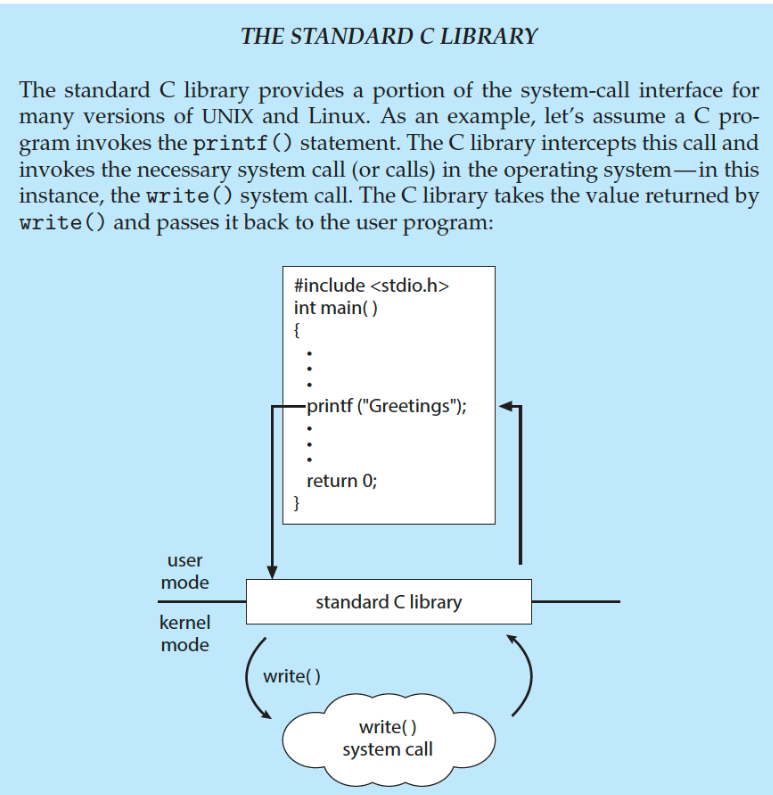
\includegraphics[width=0.5\textwidth]{images/STD_C_example.png}
    \caption{Standard C library Example}
    \label{fig:standard_c_example}
\end{figure}


\subsection{Tracing System Calls}

On Linux, the \texttt{strace} command allows users to trace the system calls executed by a running process. Internally, \texttt{strace} relies on another system call, \texttt{ptrace}, which provides the ability to trace, and potentially modify, the system call invocations of a traced process. Rather than executing a system call directly, the traced process hands control over to the tracer. The tracer can then observe the sequence of system calls, monitor timings and performance, and even modify parameters or results while the process is running. This mechanism is particularly useful for debugging, performance analysis, and understanding the behavior of programs.


\section{Operating Systems Design and Implementation}

    The design of operating systems is not a "solvable" problem in the traditional sense, but some approaches have proven successful over time. The internal structure of different operating systems can vary widely, reflecting different design philosophies, target hardware, and intended use cases.
    
    The design process should begin by defining clear goals and specifications. These are significantly affected by the choice of hardware and the type of system being developed. Generally, OS design goals can be categorized into two main areas: \emph{user goals}  and \emph{system goals}. User goals focus on making the operating system convenient to use, easy to learn, reliable, safe, and fast, ensuring that the system meets the practical needs of its users. System goals, on the other hand, emphasize that the operating system should be easy to design, implement, and maintain, as well as flexible, reliable, error-free, and efficient, focusing on the development and maintenance aspects of the system.
    Specifying and designing an operating system is a highly creative task of software engineering, requiring careful consideration of trade-offs between competing requirements and constraints.


\subsection{Policy and Mechanism}

    A fundamental principle in operating system design is the separation of \textbf{policy} and \textbf{mechanism}. Policy defines \emph{what} needs to be done and represents the decision-making aspect of system management, while mechanism defines \emph{how} to do something and represents the implementation details and tools used to enforce policies.
    
    For example, consider CPU scheduling: the policy might state "interrupt the current process after every 100 ms to allow other processes to run," while the mechanism is the hardware timer that generates interrupts at specified intervals.
    
    The separation of policy from mechanism is an important design principle because it allows maximum flexibility when policy decisions need to be changed later. In the example above, if we decide to change the time slice from 100 ms to 200 ms, we only need to modify the policy parameter without changing the underlying timer mechanism.
    
    This separation provides several advantages: policies can be modified without changing the underlying mechanisms, different policies can use the same mechanisms, changes to policies don't require extensive system modifications, and the system can adapt to different requirements and environments more easily.


\subsection{Implementation}

    Operating systems can be implemented using many different programming languages, and the choice has evolved significantly over time. Early operating systems were written entirely in assembly language for maximum performance and direct hardware control. Later, system programming languages like Algol and PL/1 were introduced, and now modern systems are predominantly written in C and C++, with some components in other languages.
    
    Contemporary operating systems typically use a mix of programming languages, each chosen for specific purposes. The lowest levels still use assembly language for boot loaders and initialization code, context switching and interrupt handling, and hardware-specific operations that require direct hardware access. The main body of the operating system is written in C, which provides a good balance between performance and portability. System programs are implemented in C, C++, and various scripting languages like PERL, Python, and shell scripts, depending on their specific requirements and the level of performance needed.
    
    The trade-off between using high-level languages versus low-level languages involves several considerations. Higher-level languages make the operating system easier to port to other hardware architectures and generally result in more maintainable and readable code. However, they typically produce slower execution compared to assembly language or optimized C code. For most modern systems, the benefits of portability and maintainability outweigh the performance costs, especially as hardware has become more powerful.
    
    An interesting approach to overcome hardware limitations is emulation, which can allow an operating system to run on non-native hardware. This technique enables compatibility across different architectures but usually comes with significant performance overhead.


\subsection{Operating System Structure}

    The princpal way to structure an operating system are:
    \begin{compactitemize}
        \item \textbf{Monolitich}
        \item \textbf{Modular}
        \item \textbf{Layered}
        \item \textbf{Microkernel}
        \item \textbf{Hybrid}
    \end{compactitemize}


\subsubsection{Monolithic Systems}

    In a monolithic operating system, the entire OS is implemented as a single large process running in a single address space. All components of the OS, including the kernel, device drivers, file system management, and system call handling, are tightly integrated and can directly call each other. This design allows for efficient communication between components and can lead to high performance since there is no overhead associated with inter-process communication (IPC) or context switching between different modules.
    
    However, monolithic systems can be complex and difficult to maintain. The tight coupling of components means that changes in one part of the system can have unintended consequences in other parts. Debugging and updating the OS can be challenging, as a bug in one component can potentially crash the entire system. Additionally, monolithic systems may not be as flexible or portable as other designs, as they are often closely tied to specific hardware architectures.
    
    Examples of monolithic operating systems include early versions of Unix and Linux. These systems have evolved over time to incorporate modular elements, but their core architecture remains largely monolithic.
    The linux architecture is an example of a monolithic system that has been designed to be modular, allowing for easier maintenance and updates while still retaining the performance benefits of a monolithic design. It can be thinked as a dynamic linking in the compilation phase.



\begin{figure}[H]
    \centering
    \begin{minipage}{0.5\textwidth}
        \centering
        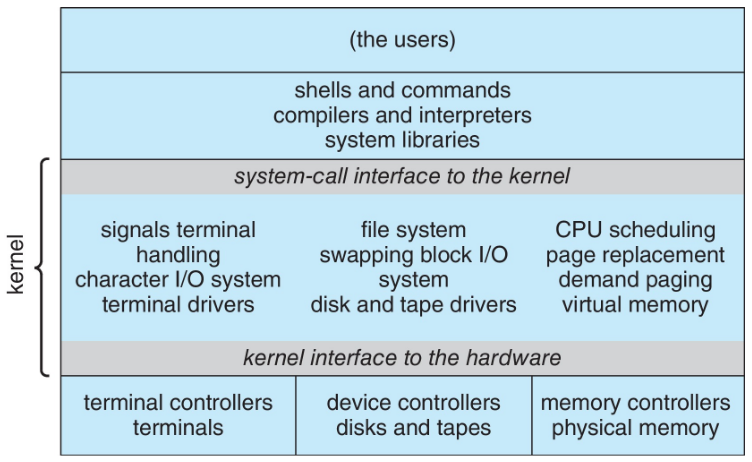
\includegraphics[width=\textwidth]{images/Traditional_unix_system_arch.png}
        \caption{Example: Traditional UNIX System Architecture}
        \label{fig:Traditional_unix_system_arch}
    \end{minipage}
    \hfill
    \begin{minipage}{0.3\textwidth}
        \centering
        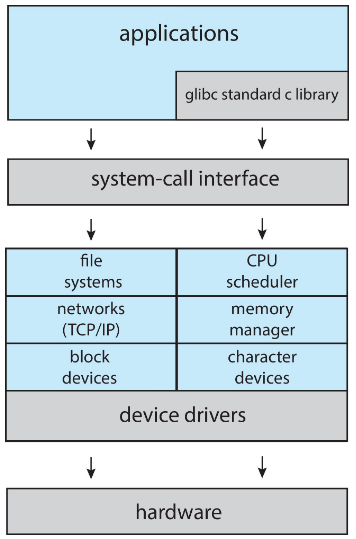
\includegraphics[width=\textwidth]{images/linux_system_architecture.png}
        \caption{Example: Linux System Architecture}
        \label{fig:Linux_system_architecture}
    \end{minipage}
    \label{fig:monolithic_examples}
\end{figure}

\subsubsection{Layered Systems}

    In a layered operating system, the OS is structured into a series of layers, each built on top of the one below it. Each layer provides a specific set of services and interacts only with the layers directly above and below it. This design promotes modularity and separation of concerns, making the system easier to understand, maintain, and modify.
    
    The lowest layer typically interacts directly with the hardware, while higher layers provide more abstract services to user applications. For example, one layer might handle memory management, while another layer manages file systems. Each layer can be developed and tested independently, which can lead to more reliable and robust systems.
    
    However, layered systems can suffer from performance overhead due to the additional abstraction layers. Each layer may introduce latency as requests are passed up and down the stack. Additionally, strict layering can sometimes lead to inefficiencies if a higher layer needs to access functionality in a lower layer that is not directly adjacent.
    
    An example of a layered operating system is the THE (Technische Hogeschool Eindhoven) operating system developed in the 1960s. Modern operating systems like macOS also incorporate layered designs in certain components, although they may not be strictly layered throughout the entire system.

    For the network passionates, the reference is the stack TCP/IP, which is structured in layers, each with specific functions and protocols.


\begin{figure}[H]
    \centering
    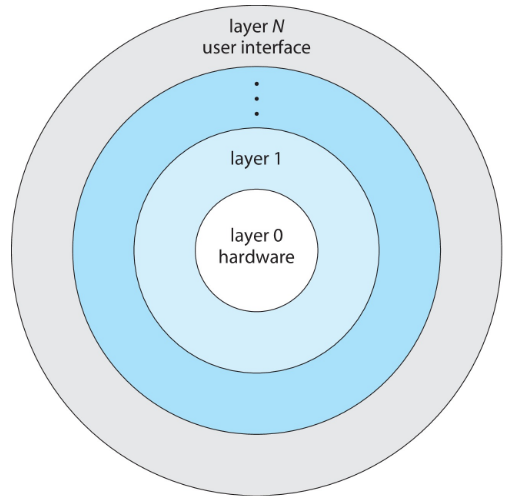
\includegraphics[width=0.3\textwidth]{images/layered_architecture.png}
    \caption{Layered Operating System Architecture}
    \label{fig:layered_architecture}
\end{figure}

\subsubsection{Microkernel Systems}

    A microkernel operating system is designed to minimize the amount of code running in kernel mode, with the goal of improving system stability, security, and maintainability. In a microkernel architecture, only the most essential functions of the operating system are implemented in the kernel, such as low-level address space management, thread management, and inter-process communication (IPC). Other services, such as device drivers, file systems, and network protocols, are implemented as user-space processes that communicate with the kernel via IPC mechanisms.
    
    This separation of concerns allows for greater modularity and flexibility. Since most of the OS services run in user space, they can be developed, tested, and updated independently of the kernel. If a user-space service crashes or misbehaves, it does not necessarily bring down the entire system, enhancing overall system reliability.
    
    However, microkernel systems can face performance challenges due to the overhead of context switching and IPC between user-space services and the kernel. The frequent communication between these components can lead to increased latency compared to monolithic systems where all components run in kernel space.
    
    Examples of microkernel operating systems include MINIX and GNU hurd. The Mach microkernel has also been influential in the development of other operating systems, such as NeXTSTEP and macOS.


\begin{figure}[H]
    \centering
    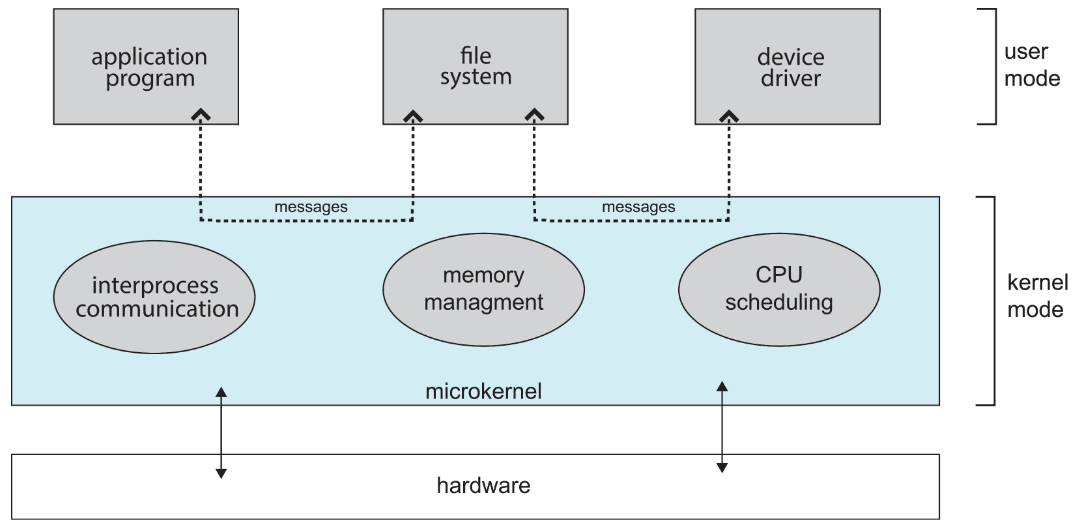
\includegraphics[width=0.6\textwidth]{images/micro_kernel_system.png}
    \caption{Micro Kernel Operating System Architecture}
    \label{fig:MICRO_kernel_system}
\end{figure}
